\section{Database}
\sloppy
\subsection{ERD}
\begin{figure}[htbp]
    \centering
    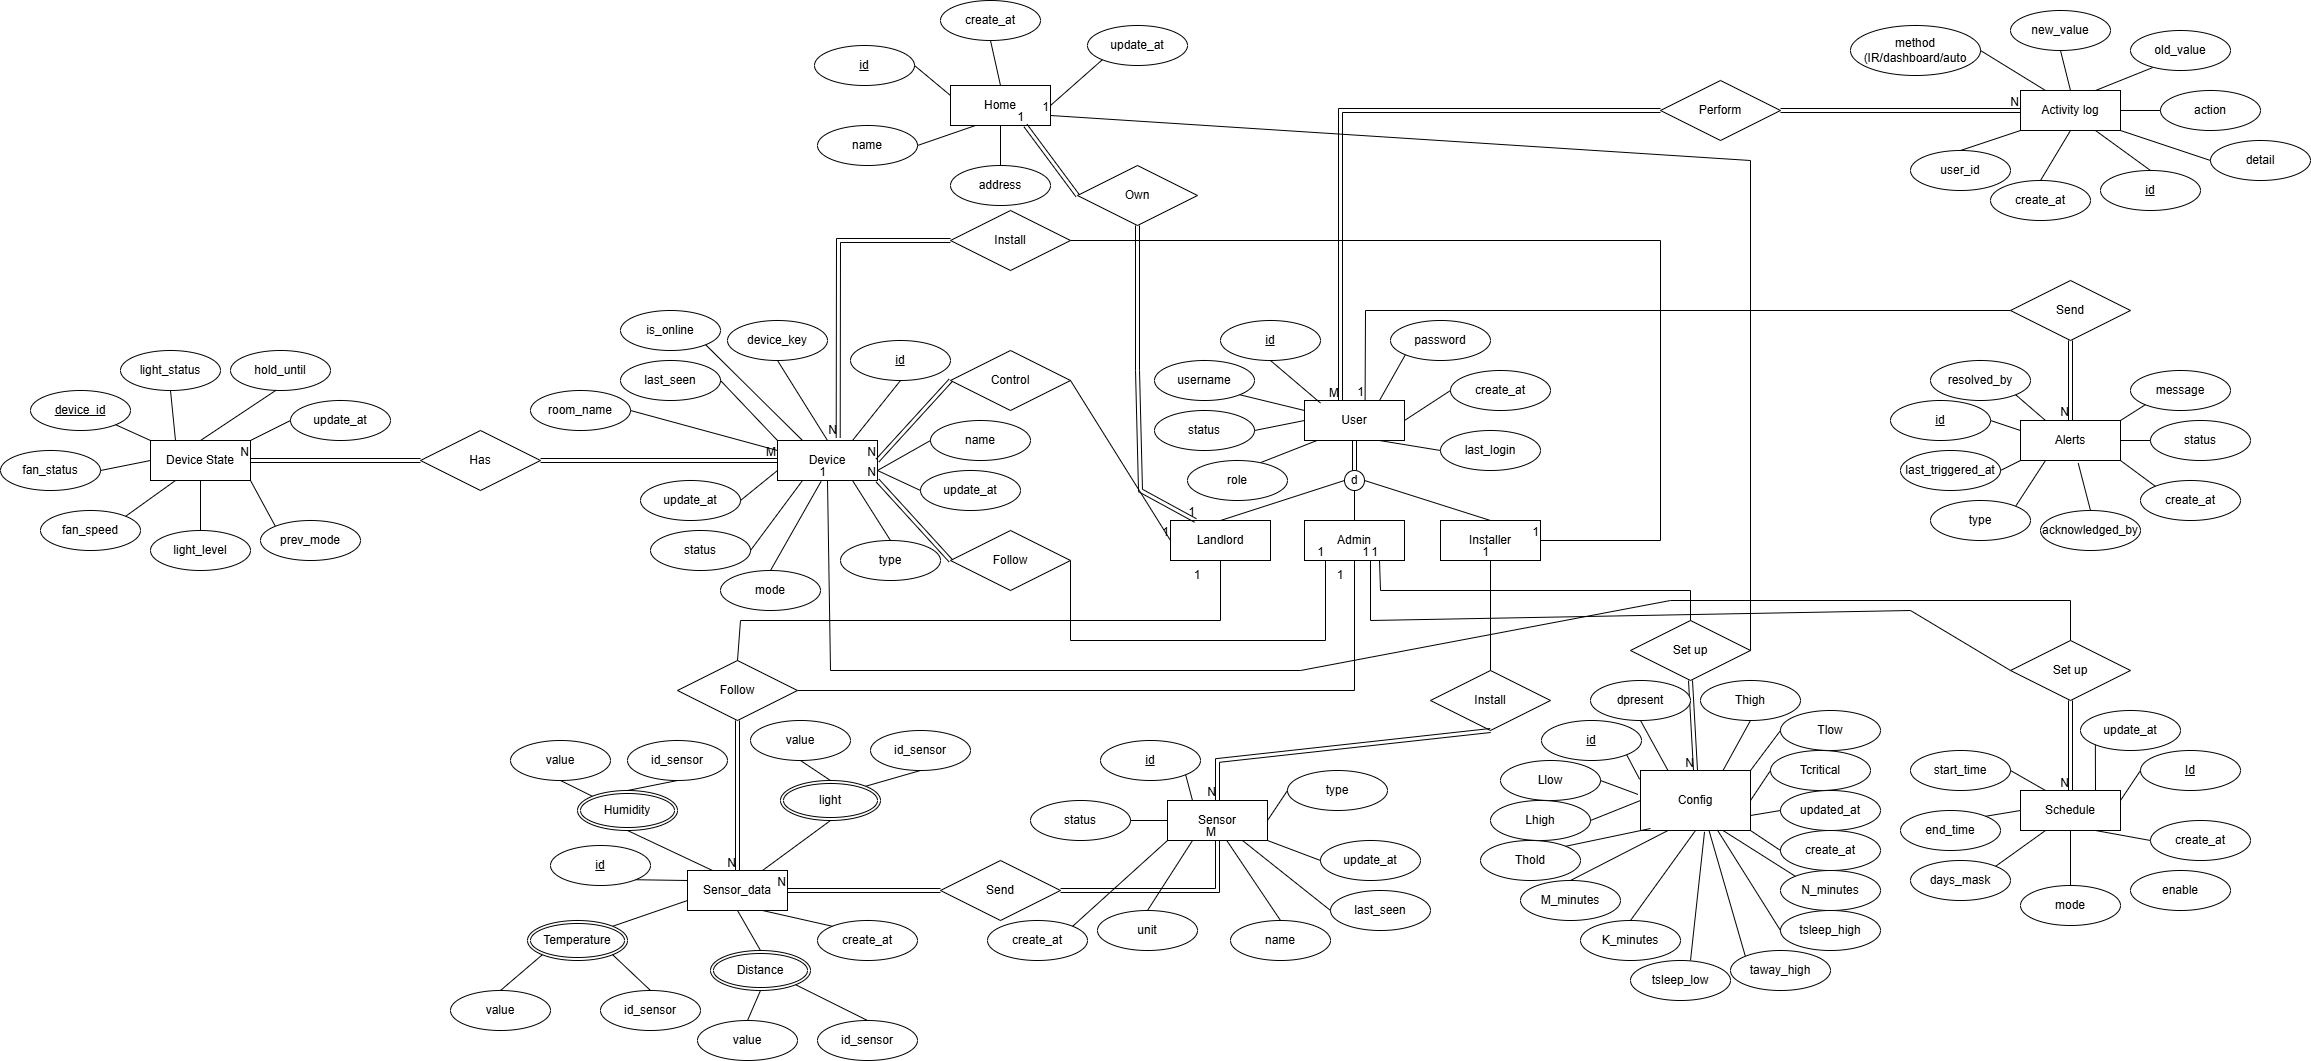
\includegraphics[width=\linewidth,height=0.78\textheight,keepaspectratio]{Images/DADN.drawio (2).png}
    \caption{ERD DATABASE}
    \label{fig:database-erd}
\end{figure}
\subsection{MAPPING}
\begin{figure}[htbp]
    \centering
    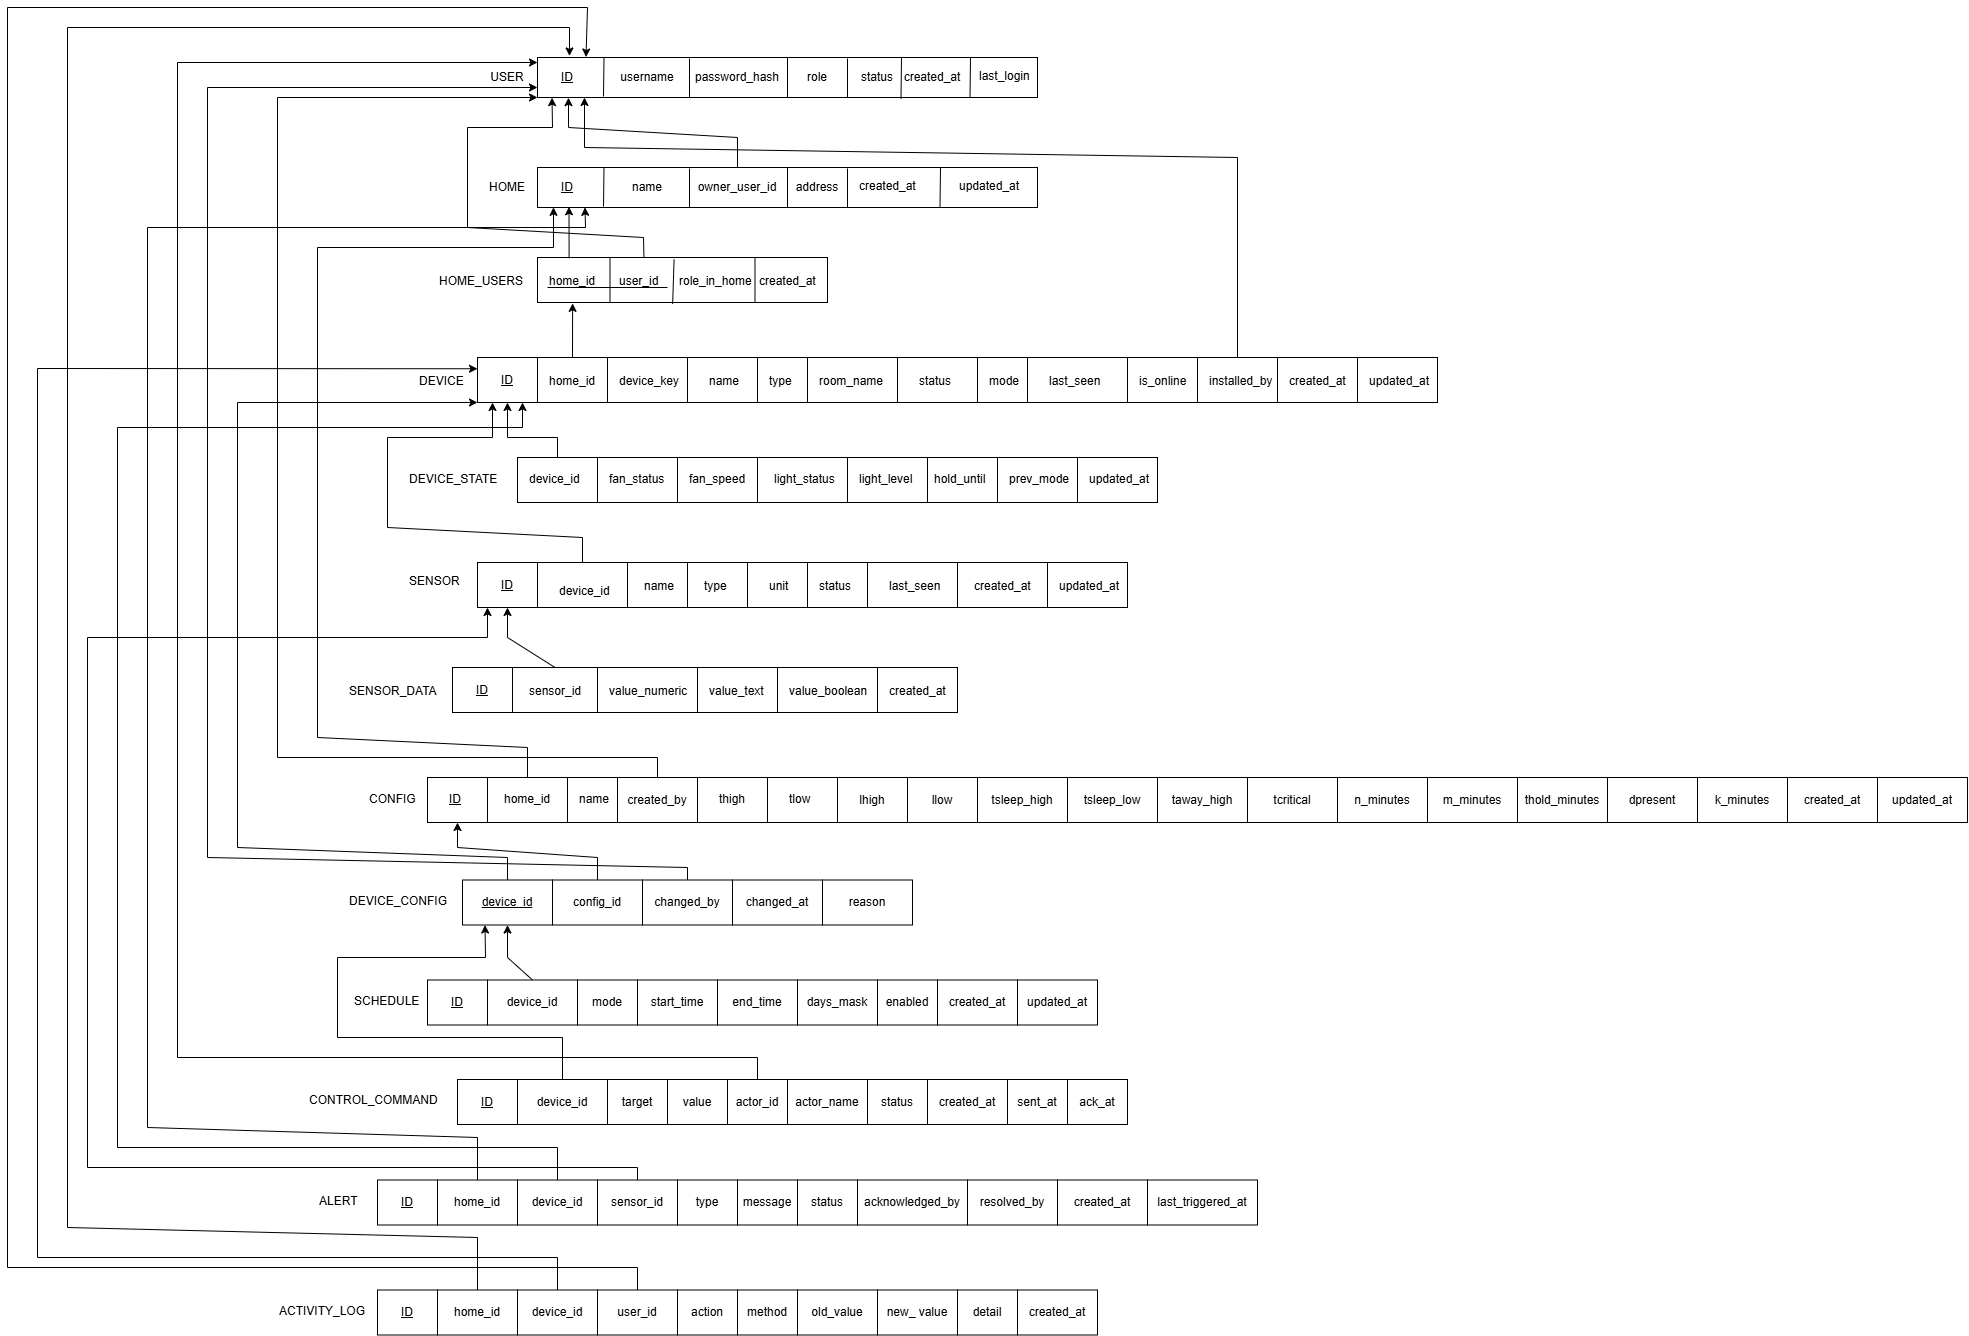
\includegraphics[width=\linewidth,height=0.78\textheight,keepaspectratio]{Images/mappingDADN.drawio.png}
    \caption{MAPPING DATABASE}
    \label{fig:database-mapping}
\end{figure}
\subsection{Đặc tả chi tiết Cơ sở dữ liệu}

Cơ sở dữ liệu của hệ thống Smart House được triển khai trên PostgreSQL và quản lý bằng Flyway migration. Thiết kế dữ liệu xoay quanh năm nhóm chính: định danh và quyền truy cập, nhà và thành viên, thiết bị và capability, telemetry và trạng thái, cấu hình tự động hóa và audit. Điểm quan trọng của mô hình là thiết bị không bị cố định bởi một vài cột trạng thái, mà được mô tả bằng \texttt{device\_capabilities}, \texttt{device\_runtime\_state}, \texttt{device\_state\_history} và \texttt{control\_commands}.

\subsubsection{Nhóm thực thể Định danh và Quyền truy cập (Identity \& Access)}

\begin{itemize}
    \item \textbf{users (Người dùng):}
    \begin{itemize}
        \item \textit{Khóa chính:} \texttt{id}.
        \item \textit{Attributes:} \texttt{username}, \texttt{password\_hash}, \texttt{role}, \texttt{status}, \texttt{must\_change\_password}, \texttt{invited\_at}, \texttt{last\_login}, \texttt{created\_at}, \texttt{updated\_at}.
        \item \textit{Ý nghĩa:} Lưu tài khoản hệ thống, vai trò toàn cục như \texttt{ADMIN}, \texttt{CUSTOMER}, \texttt{INSTALLER}, \texttt{SUPER\_ADMIN} và trạng thái tài khoản.
    \end{itemize}

    \item \textbf{user\_auth\_providers (Nhà cung cấp xác thực):}
    \begin{itemize}
        \item \textit{Khóa chính:} \texttt{id}.
        \item \textit{Khóa ngoại:} \texttt{user\_id} tham chiếu \texttt{users(id)}.
        \item \textit{Attributes:} \texttt{provider}, \texttt{provider\_user\_id}, \texttt{provider\_email}, \texttt{linked\_at}, \texttt{last\_used\_at}.
        \item \textit{Ý nghĩa:} Liên kết tài khoản với phương thức đăng nhập \texttt{LOCAL} hoặc \texttt{GOOGLE}.
    \end{itemize}

    \item \textbf{user\_refresh\_tokens (Refresh token):}
    \begin{itemize}
        \item \textit{Khóa chính:} \texttt{id}.
        \item \textit{Khóa ngoại:} \texttt{user\_id} tham chiếu \texttt{users(id)}.
        \item \textit{Attributes:} \texttt{token\_hash}, \texttt{issued\_at}, \texttt{expires\_at}, \texttt{revoked\_at}, \texttt{created\_by\_ip}, \texttt{user\_agent}.
        \item \textit{Ý nghĩa:} Quản lý phiên làm mới đăng nhập và hỗ trợ thu hồi token.
    \end{itemize}
\end{itemize}

\subsubsection{Nhóm thực thể Nhà và Thành viên (Home \& Membership)}

\begin{itemize}
    \item \textbf{homes (Nhà):}
    \begin{itemize}
        \item \textit{Khóa chính:} \texttt{id}.
        \item \textit{Khóa ngoại:} \texttt{owner\_user\_id} tham chiếu \texttt{users(id)}.
        \item \textit{Attributes:} \texttt{name}, \texttt{address}, \texttt{created\_at}, \texttt{updated\_at}.
        \item \textit{Ý nghĩa:} Xác định phạm vi logic của một nhà thông minh, làm khóa phân vùng cho thiết bị, cấu hình, cảnh báo và nhật ký.
    \end{itemize}

    \item \textbf{home\_users (Thành viên nhà):}
    \begin{itemize}
        \item \textit{Khóa chính:} \texttt{home\_id}, \texttt{user\_id}.
        \item \textit{Khóa ngoại:} \texttt{home\_id} tham chiếu \texttt{homes(id)}, \texttt{user\_id} tham chiếu \texttt{users(id)}.
        \item \textit{Attributes:} \texttt{role\_in\_home}, \texttt{allow\_profile\_activation}, \texttt{is\_primary}, \texttt{created\_at}, \texttt{updated\_at}.
        \item \textit{Ý nghĩa:} Biểu diễn quan hệ nhiều-nhiều giữa người dùng và nhà, đồng thời lưu quyền ở cấp home.
    \end{itemize}
\end{itemize}

\subsubsection{Nhóm thực thể Thiết bị và Năng lực (Device \& Capability)}

\begin{itemize}
    \item \textbf{devices (Thiết bị):}
    \begin{itemize}
        \item \textit{Khóa chính:} \texttt{id}.
        \item \textit{Khóa ngoại:} \texttt{home\_id} tham chiếu \texttt{homes(id)}, \texttt{installed\_by} tham chiếu \texttt{users(id)}.
        \item \textit{Attributes:} \texttt{device\_key}, \texttt{name}, \texttt{class}, \texttt{subtype}, \texttt{room\_name}, \texttt{status}, \texttt{last\_seen}, \texttt{is\_online}, \texttt{firmware\_version}.
        \item \textit{Ý nghĩa:} Lưu controller, actuator, sensor node, hub hoặc thiết bị khác trong nhà.
    \end{itemize}

    \item \textbf{device\_capabilities (Năng lực thiết bị):}
    \begin{itemize}
        \item \textit{Khóa chính:} \texttt{device\_id}, \texttt{capability\_code}.
        \item \textit{Khóa ngoại:} \texttt{device\_id} tham chiếu \texttt{devices(id)}.
        \item \textit{Attributes:} \texttt{value\_type}, \texttt{is\_writable}, \texttt{min\_value}, \texttt{max\_value}, \texttt{unit}, \texttt{created\_at}.
        \item \textit{Ý nghĩa:} Mô tả các khả năng như \texttt{POWER}, \texttt{SPEED}, \texttt{BRIGHTNESS}, \texttt{MODE}, \texttt{TEMPERATURE}, \texttt{HUMIDITY}, \texttt{MOTION}.
    \end{itemize}

    \item \textbf{device\_runtime\_state (Trạng thái hiện tại):}
    \begin{itemize}
        \item \textit{Khóa chính:} \texttt{device\_id}, \texttt{capability\_code}.
        \item \textit{Khóa ngoại:} \texttt{device\_id}, \texttt{capability\_code} tham chiếu \texttt{device\_capabilities}.
        \item \textit{Attributes:} \texttt{value\_boolean}, \texttt{value\_number}, \texttt{value\_text}, \texttt{updated\_at}.
        \item \textit{Ý nghĩa:} Lưu giá trị mới nhất của từng capability để dashboard hiển thị nhanh trạng thái hiện tại.
    \end{itemize}

    \item \textbf{device\_state\_history (Lịch sử trạng thái):}
    \begin{itemize}
        \item \textit{Khóa chính:} \texttt{id}.
        \item \textit{Khóa ngoại:} \texttt{device\_id}, \texttt{capability\_code} tham chiếu \texttt{device\_capabilities}; \texttt{changed\_by} tham chiếu \texttt{users(id)}.
        \item \textit{Attributes:} \texttt{value\_boolean}, \texttt{value\_number}, \texttt{value\_text}, \texttt{source}, \texttt{source\_ref\_id}, \texttt{created\_at}.
        \item \textit{Ý nghĩa:} Lưu timeline thay đổi trạng thái phục vụ lịch sử, audit và phân tích nguyên nhân.
    \end{itemize}

    \item \textbf{device\_configs (Cấu hình áp dụng cho thiết bị):}
    \begin{itemize}
        \item \textit{Khóa chính:} \texttt{device\_id}.
        \item \textit{Khóa ngoại:} \texttt{device\_id} tham chiếu \texttt{devices(id)}, \texttt{config\_id} tham chiếu \texttt{configs(id)}, \texttt{changed\_by} tham chiếu \texttt{users(id)}.
        \item \textit{Attributes:} \texttt{changed\_at}, \texttt{reason}.
        \item \textit{Ý nghĩa:} Ghi nhận cấu hình đang áp dụng cho từng thiết bị, bảo đảm thiết bị và cấu hình thuộc cùng home.
    \end{itemize}
\end{itemize}

\subsubsection{Nhóm thực thể Cảm biến và Dữ liệu (Sensor \& Telemetry)}

\begin{itemize}
    \item \textbf{sensors (Cảm biến):}
    \begin{itemize}
        \item \textit{Khóa chính:} \texttt{id}.
        \item \textit{Khóa ngoại:} \texttt{device\_id} tham chiếu \texttt{devices(id)}.
        \item \textit{Attributes:} \texttt{name}, \texttt{sensor\_kind}, \texttt{unit}, \texttt{status}, \texttt{last\_seen}, \texttt{created\_at}, \texttt{updated\_at}.
        \item \textit{Ý nghĩa:} Đại diện cho kênh đo thuộc thiết bị \texttt{SENSOR\_NODE}; hệ thống có các loại như \texttt{TEMPERATURE}, \texttt{HUMIDITY}, \texttt{LIGHT}, \texttt{MOTION}, \texttt{DISTANCE}, \texttt{SMOKE}.
    \end{itemize}

    \item \textbf{sensor\_data (Dữ liệu cảm biến):}
    \begin{itemize}
        \item \textit{Khóa chính:} \texttt{id}.
        \item \textit{Khóa ngoại:} \texttt{sensor\_id} tham chiếu \texttt{sensors(id)}.
        \item \textit{Attributes:} \texttt{value\_numeric}, \texttt{value\_text}, \texttt{value\_boolean}, \texttt{created\_at}.
        \item \textit{Ý nghĩa:} Lưu dữ liệu telemetry theo thời gian để phục vụ dashboard, biểu đồ History, cảnh báo và tự động hóa.
    \end{itemize}
\end{itemize}

\subsubsection{Nhóm thực thể Tự động hóa và Điều khiển (Automation \& Control)}

\begin{itemize}
    \item \textbf{configs (Cấu hình tự động hóa):}
    \begin{itemize}
        \item \textit{Khóa chính:} \texttt{id}.
        \item \textit{Khóa ngoại:} \texttt{home\_id} tham chiếu \texttt{homes(id)}, \texttt{created\_by} tham chiếu \texttt{users(id)}; các cột monitoring tham chiếu \texttt{devices(id)}.
        \item \textit{Attributes:} \texttt{name}, \texttt{thigh}, \texttt{tlow}, \texttt{lhigh}, \texttt{llow}, \texttt{tsleep\_high}, \texttt{tsleep\_low}, \texttt{taway\_high}, \texttt{tcritical}, \texttt{n\_minutes}, \texttt{m\_minutes}, \texttt{thold\_minutes}, \texttt{dpresent}, \texttt{k\_minutes}, \texttt{auto\_fan\_speed}, \texttt{sleep\_fan\_speed}, \texttt{away\_fan\_speed}, \texttt{is\_active}.
        \item \textit{Ý nghĩa:} Định nghĩa ngưỡng nhiệt độ, ánh sáng, thời gian giữ trạng thái, tốc độ quạt và thiết bị giám sát. Ràng buộc unique index bảo đảm mỗi home chỉ có một cấu hình active.
    \end{itemize}

    \item \textbf{schedules (Lịch thiết bị):}
    \begin{itemize}
        \item \textit{Khóa chính:} \texttt{id}.
        \item \textit{Khóa ngoại:} \texttt{device\_id}, \texttt{capability\_code} tham chiếu \texttt{device\_capabilities}; \texttt{created\_by} tham chiếu \texttt{users(id)}.
        \item \textit{Attributes:} \texttt{value\_boolean}, \texttt{value\_number}, \texttt{value\_text}, \texttt{start\_time}, \texttt{end\_time}, \texttt{days\_mask}, \texttt{enabled}, \texttt{priority}.
        \item \textit{Ý nghĩa:} Thiết lập giá trị cần áp dụng cho capability của thiết bị theo thời gian và ngày trong tuần.
    \end{itemize}

    \item \textbf{control\_commands (Lệnh điều khiển):}
    \begin{itemize}
        \item \textit{Khóa chính:} \texttt{id}.
        \item \textit{Khóa ngoại:} \texttt{device\_id} tham chiếu \texttt{devices(id)}, \texttt{actor\_id} tham chiếu \texttt{users(id)}.
        \item \textit{Attributes:} \texttt{target}, \texttt{value\_boolean}, \texttt{value\_number}, \texttt{value\_text}, \texttt{actor\_name}, \texttt{status}, \texttt{source}, \texttt{created\_at}, \texttt{sent\_at}, \texttt{ack\_at}.
        \item \textit{Ý nghĩa:} Theo dõi vòng đời lệnh từ \texttt{PENDING}, \texttt{SENT} đến \texttt{ACKED}, \texttt{FAILED} hoặc \texttt{CANCELLED}.
    \end{itemize}
\end{itemize}

\subsubsection{Nhóm thực thể Giám sát và Tích hợp (Monitoring \& Integration)}

\begin{itemize}
    \item \textbf{alerts (Cảnh báo):}
    \begin{itemize}
        \item \textit{Khóa chính:} \texttt{id}.
        \item \textit{Khóa ngoại:} \texttt{home\_id} tham chiếu \texttt{homes(id)}, \texttt{device\_id} tham chiếu \texttt{devices(id)}, \texttt{sensor\_id} tham chiếu \texttt{sensors(id)}, \texttt{acknowledged\_by} và \texttt{resolved\_by} tham chiếu \texttt{users(id)}.
        \item \textit{Attributes:} \texttt{type}, \texttt{message}, \texttt{status}, \texttt{acknowledged\_at}, \texttt{resolved\_at}, \texttt{created\_at}, \texttt{last\_triggered\_at}.
        \item \textit{Ý nghĩa:} Quản lý cảnh báo như \texttt{CRITICAL\_TEMP}, \texttt{DEVICE\_OFFLINE}, \texttt{SENSOR\_ERROR}, \texttt{HIGH\_LIGHT}, \texttt{LOW\_LIGHT}, \texttt{MOTION\_DETECTED}, \texttt{WRONG\_PASSWORD}. Vòng đời cảnh báo gồm \texttt{ACTIVE}, \texttt{ACK}, \texttt{RESOLVED}.
    \end{itemize}

    \item \textbf{activity\_logs (Nhật ký hoạt động):}
    \begin{itemize}
        \item \textit{Khóa chính:} \texttt{id}.
        \item \textit{Khóa ngoại:} \texttt{home\_id} tham chiếu \texttt{homes(id)}, \texttt{device\_id} tham chiếu \texttt{devices(id)}, \texttt{user\_id} tham chiếu \texttt{users(id)}.
        \item \textit{Attributes:} \texttt{action}, \texttt{method}, \texttt{old\_value}, \texttt{new\_value}, \texttt{detail}, \texttt{created\_at}.
        \item \textit{Ý nghĩa:} Lưu vết thao tác điều khiển, cấu hình, tự động hóa, cảnh báo và các sự kiện hệ thống để phục vụ audit.
    \end{itemize}

    \item \textbf{outbox\_event (Sự kiện tích hợp):}
    \begin{itemize}
        \item \textit{Khóa chính:} \texttt{id}.
        \item \textit{Attributes:} \texttt{aggregate\_type}, \texttt{aggregate\_id}, \texttt{event\_type}, \texttt{payload}, \texttt{status}, \texttt{retry\_count}, \texttt{last\_error}, \texttt{created\_at}, \texttt{published\_at}.
        \item \textit{Ý nghĩa:} Lưu sự kiện cần phát sang RabbitMQ, hỗ trợ retry và theo dõi trạng thái publish.
    \end{itemize}
\end{itemize}

\subsubsection{Quan hệ dữ liệu chính}

\begin{itemize}
    \item Một \texttt{users} được phép sở hữu nhiều \texttt{homes} và tham gia nhiều home qua \texttt{home\_users}.
    \item Một \texttt{homes} có nhiều \texttt{devices}, \texttt{configs}, \texttt{alerts} và \texttt{activity\_logs}.
    \item Một \texttt{devices} có nhiều \texttt{device\_capabilities}, \texttt{sensors}, \texttt{schedules}, \texttt{control\_commands}, \texttt{device\_state\_history}.
    \item Một capability của thiết bị có tối đa một bản ghi trạng thái hiện tại trong \texttt{device\_runtime\_state}.
    \item Một \texttt{sensors} có nhiều \texttt{sensor\_data}; dữ liệu này là đầu vào cho dashboard, lịch sử, cảnh báo và tự động hóa.
    \item Một \texttt{configs} liên kết tới các thiết bị giám sát thông qua \texttt{monitoring\_temperature\_device\_id}, \texttt{monitoring\_humidity\_device\_id}, \texttt{monitoring\_light\_sensor\_device\_id}, \texttt{monitoring\_motion\_device\_id}, \texttt{monitoring\_fan\_device\_id}, \texttt{monitoring\_light\_device\_id}.
    \item \texttt{alerts} và \texttt{activity\_logs} liên kết ngược về home, device, sensor hoặc user để truy vết nguyên nhân.
\end{itemize}

\subsubsection{Các ràng buộc và chỉ mục quan trọng}

\begin{itemize}
    \item \texttt{device\_key} là duy nhất, giúp gateway và thiết bị định danh đúng thiết bị.
    \item Các bảng lưu giá trị như \texttt{sensor\_data}, \texttt{control\_commands}, \texttt{schedules}, \texttt{device\_runtime\_state} yêu cầu đúng một kiểu giá trị trong ba cột boolean, number hoặc text.
    \item Trigger database kiểm tra sensor chỉ gắn với thiết bị \texttt{SENSOR\_NODE}, lệnh và runtime state phải khớp capability, alert phải thuộc đúng home của device hoặc sensor.
    \item Index trên \texttt{activity\_logs}, \texttt{sensor\_data}, \texttt{control\_commands}, \texttt{alerts} hỗ trợ truy vấn dashboard, history, long-poll command và audit.
    \item Unique index \texttt{uq\_configs\_one\_active\_per\_home} bảo đảm một home chỉ có một profile active tại một thời điểm.
\end{itemize}

\subsubsection{Cấu hình kết nối, migration và seed data}

\begin{itemize}
    \item Backend kết nối PostgreSQL qua \texttt{spring.datasource.url}, \texttt{spring.datasource.username}, \texttt{spring.datasource.password} trong \texttt{backend/src/main/resources/application.properties}. Các biến môi trường tương ứng là \texttt{DB\_URL}, \texttt{DB\_USERNAME}, \texttt{DB\_PASSWORD}.
    \item Khi chạy bằng Docker Compose, service \texttt{db} dùng image \texttt{postgres:18-alpine}, expose cổng \texttt{5432:5432} và lưu dữ liệu vào volume \texttt{postgres\_data}.
    \item Flyway được bật qua \texttt{spring.flyway.enabled}; thư mục migration là \texttt{classpath:db/migration}.
    \item \texttt{V1\_\_init.sql} tạo enum, bảng, trigger, index, ràng buộc và dữ liệu mẫu. Các migration \texttt{V2} đến \texttt{V5} bổ sung cột \texttt{source} cho lệnh điều khiển và index phục vụ realtime command, activity log, audit dashboard.
\end{itemize}

\subsubsection{Mapping database - entity - repository - service}

{\scriptsize
\setlength{\tabcolsep}{2pt}
\renewcommand{\arraystretch}{1.12}
\begin{longtable}{|p{0.18\textwidth}|p{0.24\textwidth}|p{0.25\textwidth}|p{0.25\textwidth}|}
\caption{Mapping database, entity, repository và service}\\
\hline
\textbf{Bảng} & \textbf{Entity} & \textbf{Repository} & \textbf{Service liên quan} \\
\hline
\endfirsthead
\hline
\textbf{Bảng} & \textbf{Entity} & \textbf{Repository} & \textbf{Service liên quan} \\
\hline
\endhead
\texttt{users} & \texttt{UserEntity.java} & \texttt{UserRepository.java} & \texttt{AuthenticationService}, \texttt{UserProvisioningService}, \texttt{ProfileService} \\
\hline
\texttt{user\_auth\_providers} & \texttt{UserAuthProviderEntity.java} & \texttt{UserAuthProvider}\newline\texttt{Repository.java} & \texttt{UserAuthProviderLinker}, \texttt{AuthenticationService} \\
\hline
\texttt{user\_refresh\_tokens} & \texttt{UserRefreshTokenEntity.java} & \texttt{UserRefreshToken}\newline\texttt{Repository.java} & \texttt{RefreshTokenService}, \texttt{TokenRefreshFacade} \\
\hline
\texttt{homes} & \texttt{HomeEntity.java} & \texttt{HomeRepository.java} & \texttt{HomeAccessService}, \texttt{HomeProfileService} \\
\hline
\texttt{home\_users} & \texttt{HomeUserEntity.java} & \texttt{HomeUserRepository.java} & \texttt{HomeUserManagementService}, \texttt{HomeMembershipService} \\
\hline
\texttt{devices} & \texttt{DeviceEntity.java} & \texttt{DeviceRepository.java} & \texttt{DeviceService}, \texttt{DeviceControlService}, \texttt{DashboardService} \\
\hline
\texttt{device\_capabilities} & \texttt{DeviceCapabilityEntity.java} & \texttt{DeviceCapability}\newline\texttt{Repository.java} & \texttt{DeviceTargetPolicy}, \texttt{DeviceRuntimeStateService} \\
\hline
\texttt{device\_runtime\_state} & \texttt{DeviceRuntimeStateEntity.java} & \texttt{DeviceRuntimeState}\newline\texttt{Repository.java} & \texttt{DeviceRuntimeStateService}, \texttt{DashboardRealtimeService} \\
\hline
\texttt{device\_state\_history} & \texttt{DeviceStateHistoryEntity.java} & \texttt{DeviceStateHistory}\newline\texttt{Repository.java} & \texttt{DeviceStateHistoryService}, \texttt{TelemetryHistoryService} \\
\hline
\texttt{sensors} & \texttt{SensorEntity.java} & \texttt{SensorRepository.java} & \texttt{TelemetryPersistenceService}, \texttt{SensorSnapshotService} \\
\hline
\texttt{sensor\_data} & \texttt{SensorDataEntity.java} & \texttt{SensorDataRepository.java} & \texttt{TelemetryPersistenceService}, \texttt{TelemetryHistoryService} \\
\hline
\texttt{configs} & \texttt{ConfigEntity.java} & \texttt{ConfigRepository.java} & \texttt{ConfigService}, \texttt{TelemetryAutomationService}, \texttt{ModeAutomationService} \\
\hline
\texttt{schedules} & \texttt{ScheduleEntity.java} & \texttt{ScheduleRepository.java} & \texttt{ScheduleService}, \texttt{DeviceScheduleScheduler} \\
\hline
\texttt{control\_commands} & \texttt{ControlCommandEntity.java} & \texttt{ControlCommandRepository.java} & \texttt{ControlCommandService}, \texttt{DeviceCommandExecutionService} \\
\hline
\texttt{alerts} & \texttt{AlertEntity.java} & \texttt{AlertRepository.java} & \texttt{AlertService}, \texttt{TelemetryAlertService}, \texttt{DeviceOfflineMonitorService} \\
\hline
\texttt{activity\_logs} & \texttt{ActivityLogEntity.java} & \texttt{ActivityLogRepository.java} & \texttt{ActivityLogService}, \texttt{AuditDashboardService}, \texttt{AuditFilterService} \\
\hline
\texttt{outbox\_event} & \texttt{OutboxEventEntity.java} & \texttt{OutboxEventRepository.java} & \texttt{UserEventOutboxService}, \texttt{OutboxEventPublisher} \\
\hline
\end{longtable}
}
